\documentclass[1p]{elsarticle_modified}
%\bibliographystyle{elsarticle-num}

%\usepackage[colorlinks]{hyperref}
%\usepackage{abbrmath_seonhwa} %\Abb, \Ascr, \Acal ,\Abf, \Afrak
\usepackage{amsfonts}
\usepackage{amssymb}
\usepackage{amsmath}
\usepackage{amsthm}
\usepackage{scalefnt}
\usepackage{amsbsy}
\usepackage{kotex}
\usepackage{caption}
\usepackage{subfig}
\usepackage{color}
\usepackage{graphicx}
\usepackage{xcolor} %% white, black, red, green, blue, cyan, magenta, yellow
\usepackage{float}
\usepackage{setspace}
\usepackage{hyperref}

\usepackage{tikz}
\usetikzlibrary{arrows}

\usepackage{multirow}
\usepackage{array} % fixed length table
\usepackage{hhline}

%%%%%%%%%%%%%%%%%%%%%
\makeatletter
\renewcommand*\env@matrix[1][\arraystretch]{%
	\edef\arraystretch{#1}%
	\hskip -\arraycolsep
	\let\@ifnextchar\new@ifnextchar
	\array{*\c@MaxMatrixCols c}}
\makeatother %https://tex.stackexchange.com/questions/14071/how-can-i-increase-the-line-spacing-in-a-matrix
%%%%%%%%%%%%%%%

\usepackage[normalem]{ulem}

\newcommand{\msout}[1]{\ifmmode\text{\sout{\ensuremath{#1}}}\else\sout{#1}\fi}
%SOURCE: \msout is \stkout macro in https://tex.stackexchange.com/questions/20609/strikeout-in-math-mode

\newcommand{\cancel}[1]{
	\ifmmode
	{\color{red}\msout{#1}}
	\else
	{\color{red}\sout{#1}}
	\fi
}

\newcommand{\add}[1]{
	{\color{blue}\uwave{#1}}
}

\newcommand{\replace}[2]{
	\ifmmode
	{\color{red}\msout{#1}}{\color{blue}\uwave{#2}}
	\else
	{\color{red}\sout{#1}}{\color{blue}\uwave{#2}}
	\fi
}

\newcommand{\Sol}{\mathcal{S}} %segment
\newcommand{\D}{D} %diagram
\newcommand{\A}{\mathcal{A}} %arc


%%%%%%%%%%%%%%%%%%%%%%%%%%%%%5 test

\def\sl{\operatorname{\textup{SL}}(2,\Cbb)}
\def\psl{\operatorname{\textup{PSL}}(2,\Cbb)}
\def\quan{\mkern 1mu \triangleright \mkern 1mu}

\theoremstyle{definition}
\newtheorem{thm}{Theorem}[section]
\newtheorem{prop}[thm]{Proposition}
\newtheorem{lem}[thm]{Lemma}
\newtheorem{ques}[thm]{Question}
\newtheorem{cor}[thm]{Corollary}
\newtheorem{defn}[thm]{Definition}
\newtheorem{exam}[thm]{Example}
\newtheorem{rmk}[thm]{Remark}
\newtheorem{alg}[thm]{Algorithm}

\newcommand{\I}{\sqrt{-1}}
\begin{document}

%\begin{frontmatter}
%
%\title{Boundary parabolic representations of knots up to 8 crossings}
%
%%% Group authors per affiliation:
%\author{Yunhi Cho} 
%\address{Department of Mathematics, University of Seoul, Seoul, Korea}
%\ead{yhcho@uos.ac.kr}
%
%
%\author{Seonhwa Kim} %\fnref{s_kim}}
%\address{Center for Geometry and Physics, Institute for Basic Science, Pohang, 37673, Korea}
%\ead{ryeona17@ibs.re.kr}
%
%\author{Hyuk Kim}
%\address{Department of Mathematical Sciences, Seoul National University, Seoul 08826, Korea}
%\ead{hyukkim@snu.ac.kr}
%
%\author{Seokbeom Yoon}
%\address{Department of Mathematical Sciences, Seoul National University, Seoul, 08826,  Korea}
%\ead{sbyoon15@snu.ac.kr}
%
%\begin{abstract}
%We find all boundary parabolic representation of knots up to 8 crossings.
%
%\end{abstract}
%\begin{keyword}
%    \MSC[2010] 57M25 
%\end{keyword}
%
%\end{frontmatter}

%\linenumbers
%\tableofcontents
%
\newcommand\colored[1]{\textcolor{white}{\rule[-0.35ex]{0.8em}{1.4ex}}\kern-0.8em\color{red} #1}%
%\newcommand\colored[1]{\textcolor{white}{ #1}\kern-2.17ex	\textcolor{white}{ #1}\kern-1.81ex	\textcolor{white}{ #1}\kern-2.15ex\color{red}#1	}

{\Large $\underline{12n_{0255}~(K12n_{0255})}$}

\setlength{\tabcolsep}{10pt}
\renewcommand{\arraystretch}{1.6}
\vspace{1cm}\begin{tabular}{m{100pt}>{\centering\arraybackslash}m{274pt}}
\multirow{5}{120pt}{
	\centering
	\includegraphics[width=112pt]{../../../GIT/diagram.site/Diagrams/png/2344_12n_0255.png}\\
\ \ \ A knot diagram\footnotemark}&
\allowdisplaybreaks
\textbf{Linearized knot diagam} \\
\cline{2-2}
 &
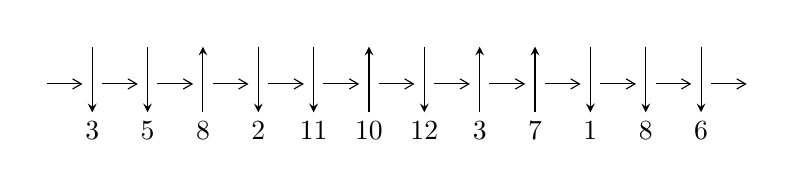
\begin{tikzpicture}[x=20pt, y=17pt]
	% nodes
	\node (C0) at (0, 0) {};
	\node (C1) at (1, 0) {};
	\node (C1U) at (1, +1) {};
	\node (C1D) at (1, -1) {3};

	\node (C2) at (2, 0) {};
	\node (C2U) at (2, +1) {};
	\node (C2D) at (2, -1) {5};

	\node (C3) at (3, 0) {};
	\node (C3U) at (3, +1) {};
	\node (C3D) at (3, -1) {8};

	\node (C4) at (4, 0) {};
	\node (C4U) at (4, +1) {};
	\node (C4D) at (4, -1) {2};

	\node (C5) at (5, 0) {};
	\node (C5U) at (5, +1) {};
	\node (C5D) at (5, -1) {11};

	\node (C6) at (6, 0) {};
	\node (C6U) at (6, +1) {};
	\node (C6D) at (6, -1) {10};

	\node (C7) at (7, 0) {};
	\node (C7U) at (7, +1) {};
	\node (C7D) at (7, -1) {12};

	\node (C8) at (8, 0) {};
	\node (C8U) at (8, +1) {};
	\node (C8D) at (8, -1) {3};

	\node (C9) at (9, 0) {};
	\node (C9U) at (9, +1) {};
	\node (C9D) at (9, -1) {7};

	\node (C10) at (10, 0) {};
	\node (C10U) at (10, +1) {};
	\node (C10D) at (10, -1) {1};

	\node (C11) at (11, 0) {};
	\node (C11U) at (11, +1) {};
	\node (C11D) at (11, -1) {8};

	\node (C12) at (12, 0) {};
	\node (C12U) at (12, +1) {};
	\node (C12D) at (12, -1) {6};
	\node (C13) at (13, 0) {};

	% arrows
	\draw[->,>={angle 60}]
	(C0) edge (C1) (C1) edge (C2) (C2) edge (C3) (C3) edge (C4) (C4) edge (C5) (C5) edge (C6) (C6) edge (C7) (C7) edge (C8) (C8) edge (C9) (C9) edge (C10) (C10) edge (C11) (C11) edge (C12) (C12) edge (C13) ;	\draw[->,>=stealth]
	(C1U) edge (C1D) (C2U) edge (C2D) (C3D) edge (C3U) (C4U) edge (C4D) (C5U) edge (C5D) (C6D) edge (C6U) (C7U) edge (C7D) (C8D) edge (C8U) (C9D) edge (C9U) (C10U) edge (C10D) (C11U) edge (C11D) (C12U) edge (C12D) ;
	\end{tikzpicture} \\
\hhline{~~} \\& 
\textbf{Solving Sequence} \\ \cline{2-2} 
 &
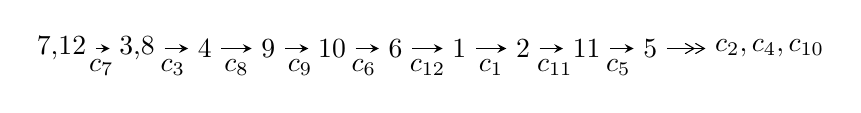
\begin{tikzpicture}[x=23pt, y=7pt]
	% node
	\node (A0) at (-1/8, 0) {7,12};
	\node (A1) at (17/16, 0) {3,8};
	\node (A2) at (17/8, 0) {4};
	\node (A3) at (25/8, 0) {9};
	\node (A4) at (33/8, 0) {10};
	\node (A5) at (41/8, 0) {6};
	\node (A6) at (49/8, 0) {1};
	\node (A7) at (57/8, 0) {2};
	\node (A8) at (65/8, 0) {11};
	\node (A9) at (73/8, 0) {5};
	\node (C1) at (1/2, -1) {$c_{7}$};
	\node (C2) at (13/8, -1) {$c_{3}$};
	\node (C3) at (21/8, -1) {$c_{8}$};
	\node (C4) at (29/8, -1) {$c_{9}$};
	\node (C5) at (37/8, -1) {$c_{6}$};
	\node (C6) at (45/8, -1) {$c_{12}$};
	\node (C7) at (53/8, -1) {$c_{1}$};
	\node (C8) at (61/8, -1) {$c_{11}$};
	\node (C9) at (69/8, -1) {$c_{5}$};
	\node (A10) at (11, 0) {$c_{2},c_{4},c_{10}$};

	% edge
	\draw[->,>=stealth]	
	(A0) edge (A1) (A1) edge (A2) (A2) edge (A3) (A3) edge (A4) (A4) edge (A5) (A5) edge (A6) (A6) edge (A7) (A7) edge (A8) (A8) edge (A9) ;
	\draw[->>,>={angle 60}]	
	(A9) edge (A10);
\end{tikzpicture} \\ 

\end{tabular} \\

\footnotetext{
The image of knot diagram is generated by the software ``\textbf{Draw programme}" developed by Andrew Bartholomew(\url{http://www.layer8.co.uk/maths/draw/index.htm\#Running-draw}), where we modified some parts for our purpose(\url{https://github.com/CATsTAILs/LinksPainter}).
}\phantom \\ \newline 
\centering \textbf{Ideals for irreducible components\footnotemark of $X_{\text{par}}$} 
 
\begin{align*}
I^u_{1}&=\langle 
1.59660\times10^{327} u^{87}-4.52798\times10^{327} u^{86}+\cdots+9.40594\times10^{329} b+8.06817\times10^{330},\\
\phantom{I^u_{1}}&\phantom{= \langle  }-1.52962\times10^{329} u^{87}+3.20986\times10^{329} u^{86}+\cdots+4.75941\times10^{331} a-3.66335\times10^{331},\\
\phantom{I^u_{1}}&\phantom{= \langle  }u^{88}-2 u^{87}+\cdots-4968 u-1771\rangle \\
I^u_{2}&=\langle 
4 u^8+u^6-4 u^5+2 u^4-5 u^3- u^2+7 b+u+3,\;4 u^8+7 u^7+15 u^6+10 u^5+16 u^4+9 u^3+13 u^2+7 a+u+3,\\
\phantom{I^u_{2}}&\phantom{= \langle  }u^9+u^8+2 u^7+u^6+3 u^5+u^4+2 u^3+u-1\rangle \\
I^u_{3}&=\langle 
-4 u^{15}-30 u^{13}+\cdots+b+8,\;2 u^{15}+14 u^{13}+\cdots+a-7,\;u^{16}+8 u^{14}+\cdots-3 u+1\rangle \\
\\
\end{align*}
\raggedright * 3 irreducible components of $\dim_{\mathbb{C}}=0$, with total 113 representations.\\
\footnotetext{All coefficients of polynomials are rational numbers. But the coefficients are sometimes approximated in decimal forms when there is not enough margin.}
\newpage
\renewcommand{\arraystretch}{1}
\centering \section*{I. $I^u_{1}= \langle 1.60\times10^{327} u^{87}-4.53\times10^{327} u^{86}+\cdots+9.41\times10^{329} b+8.07\times10^{330},\;-1.53\times10^{329} u^{87}+3.21\times10^{329} u^{86}+\cdots+4.76\times10^{331} a-3.66\times10^{331},\;u^{88}-2 u^{87}+\cdots-4968 u-1771 \rangle$}
\flushleft \textbf{(i) Arc colorings}\\
\begin{tabular}{m{7pt} m{180pt} m{7pt} m{180pt} }
\flushright $a_{7}=$&$\begin{pmatrix}1\\0\end{pmatrix}$ \\
\flushright $a_{12}=$&$\begin{pmatrix}0\\u\end{pmatrix}$ \\
\flushright $a_{3}=$&$\begin{pmatrix}0.00321388 u^{87}-0.00674424 u^{86}+\cdots-11.3051 u+0.769708\\-0.00169744 u^{87}+0.00481396 u^{86}+\cdots-12.5593 u-8.57774\end{pmatrix}$ \\
\flushright $a_{8}=$&$\begin{pmatrix}1\\u^2\end{pmatrix}$ \\
\flushright $a_{4}=$&$\begin{pmatrix}0.00233250 u^{87}-0.00315963 u^{86}+\cdots-27.9840 u-7.24757\\-0.00137179 u^{87}+0.00300797 u^{86}+\cdots-5.06937 u-5.35127\end{pmatrix}$ \\
\flushright $a_{9}=$&$\begin{pmatrix}0.00153178 u^{87}-0.00266896 u^{86}+\cdots-23.2890 u-2.25667\\-0.00185920 u^{87}+0.00347861 u^{86}+\cdots+19.0323 u+2.82726\end{pmatrix}$ \\
\flushright $a_{10}=$&$\begin{pmatrix}-0.000327420 u^{87}+0.000809657 u^{86}+\cdots-4.25669 u+0.570591\\-0.00185920 u^{87}+0.00347861 u^{86}+\cdots+19.0323 u+2.82726\end{pmatrix}$ \\
\flushright $a_{6}=$&$\begin{pmatrix}0.000561869 u^{87}-0.00155079 u^{86}+\cdots-8.50672 u-1.66797\\-0.000861961 u^{87}+0.00450290 u^{86}+\cdots-41.5986 u-14.7883\end{pmatrix}$ \\
\flushright $a_{1}=$&$\begin{pmatrix}-0.000151726 u^{87}+0.00147337 u^{86}+\cdots+0.554564 u-2.10313\\-0.00150768 u^{87}+0.00204381 u^{86}+\cdots+20.3844 u+3.14401\end{pmatrix}$ \\
\flushright $a_{2}=$&$\begin{pmatrix}-0.00467421 u^{87}+0.0109893 u^{86}+\cdots+15.1651 u-4.16426\\0.00197314 u^{87}-0.00700781 u^{86}+\cdots+30.3390 u+12.6165\end{pmatrix}$ \\
\flushright $a_{11}=$&$\begin{pmatrix}u\\u^3+u\end{pmatrix}$ \\
\flushright $a_{5}=$&$\begin{pmatrix}0.000632418 u^{87}-0.00298532 u^{86}+\cdots+1.50043 u+2.65355\\-1.09936\times10^{-6} u^{87}+0.00267945 u^{86}+\cdots-37.8923 u-12.7574\end{pmatrix}$\\&\end{tabular}
\flushleft \textbf{(ii) Obstruction class $= -1$}\\~\\
\flushleft \textbf{(iii) Cusp Shapes $= 0.0135860 u^{87}-0.0234158 u^{86}+\cdots-148.906 u-31.3158$}\\~\\
\newpage\renewcommand{\arraystretch}{1}
\flushleft \textbf{(iv) u-Polynomials at the component}\newline \\
\begin{tabular}{m{50pt}|m{274pt}}
Crossings & \hspace{64pt}u-Polynomials at each crossing \\
\hline $$\begin{aligned}c_{1}\end{aligned}$$&$\begin{aligned}
&u^{88}+36 u^{87}+\cdots+9016 u+2401
\end{aligned}$\\
\hline $$\begin{aligned}c_{2},c_{4}\end{aligned}$$&$\begin{aligned}
&u^{88}-16 u^{87}+\cdots+504 u-49
\end{aligned}$\\
\hline $$\begin{aligned}c_{3},c_{8}\end{aligned}$$&$\begin{aligned}
&u^{88}+u^{87}+\cdots+14336 u+25088
\end{aligned}$\\
\hline $$\begin{aligned}c_{5}\end{aligned}$$&$\begin{aligned}
&u^{88}- u^{87}+\cdots+8558243 u-2435537
\end{aligned}$\\
\hline $$\begin{aligned}c_{6},c_{9}\end{aligned}$$&$\begin{aligned}
&u^{88}+3 u^{87}+\cdots-1497 u-181
\end{aligned}$\\
\hline $$\begin{aligned}c_{7},c_{11}\end{aligned}$$&$\begin{aligned}
&u^{88}+2 u^{87}+\cdots+4968 u-1771
\end{aligned}$\\
\hline $$\begin{aligned}c_{10}\end{aligned}$$&$\begin{aligned}
&u^{88}-14 u^{87}+\cdots-5848 u+1043
\end{aligned}$\\
\hline $$\begin{aligned}c_{12}\end{aligned}$$&$\begin{aligned}
&u^{88}-4 u^{87}+\cdots+2 u-1
\end{aligned}$\\
\hline
\end{tabular}\\~\\
\newpage\renewcommand{\arraystretch}{1}
\flushleft \textbf{(v) Riley Polynomials at the component}\newline \\
\begin{tabular}{m{50pt}|m{274pt}}
Crossings & \hspace{64pt}Riley Polynomials at each crossing \\
\hline $$\begin{aligned}c_{1}\end{aligned}$$&$\begin{aligned}
&y^{88}+48 y^{87}+\cdots-1539089020 y+5764801
\end{aligned}$\\
\hline $$\begin{aligned}c_{2},c_{4}\end{aligned}$$&$\begin{aligned}
&y^{88}-36 y^{87}+\cdots-9016 y+2401
\end{aligned}$\\
\hline $$\begin{aligned}c_{3},c_{8}\end{aligned}$$&$\begin{aligned}
&y^{88}-63 y^{87}+\cdots-10096214016 y+629407744
\end{aligned}$\\
\hline $$\begin{aligned}c_{5}\end{aligned}$$&$\begin{aligned}
&y^{88}+33 y^{87}+\cdots+85934090519941 y+5931840478369
\end{aligned}$\\
\hline $$\begin{aligned}c_{6},c_{9}\end{aligned}$$&$\begin{aligned}
&y^{88}+49 y^{87}+\cdots-883509 y+32761
\end{aligned}$\\
\hline $$\begin{aligned}c_{7},c_{11}\end{aligned}$$&$\begin{aligned}
&y^{88}+70 y^{87}+\cdots+39623986 y+3136441
\end{aligned}$\\
\hline $$\begin{aligned}c_{10}\end{aligned}$$&$\begin{aligned}
&y^{88}+2 y^{87}+\cdots+12594048 y+1087849
\end{aligned}$\\
\hline $$\begin{aligned}c_{12}\end{aligned}$$&$\begin{aligned}
&y^{88}-16 y^{87}+\cdots+6 y+1
\end{aligned}$\\
\hline
\end{tabular}\\~\\
\newpage\flushleft \textbf{(vi) Complex Volumes and Cusp Shapes}
$$\begin{array}{c|c|c}  
\text{Solutions to }I^u_{1}& \I (\text{vol} + \sqrt{-1}CS) & \text{Cusp shape}\\
 \hline 
\begin{aligned}
u &= \phantom{-}0.805310 + 0.589984 I \\
a &= \phantom{-}0.054018 - 0.595613 I \\
b &= -0.564062 + 0.307745 I\end{aligned}
 & -0.95191 - 5.34222 I & \phantom{-0.000000 } 0 \\ \hline\begin{aligned}
u &= \phantom{-}0.805310 - 0.589984 I \\
a &= \phantom{-}0.054018 + 0.595613 I \\
b &= -0.564062 - 0.307745 I\end{aligned}
 & -0.95191 + 5.34222 I & \phantom{-0.000000 } 0 \\ \hline\begin{aligned}
u &= -0.992163 + 0.083390 I \\
a &= \phantom{-}0.98711 + 1.32599 I \\
b &= \phantom{-}1.43776 + 0.20661 I\end{aligned}
 & -3.57000 + 4.86222 I & \phantom{-0.000000 } 0 \\ \hline\begin{aligned}
u &= -0.992163 - 0.083390 I \\
a &= \phantom{-}0.98711 - 1.32599 I \\
b &= \phantom{-}1.43776 - 0.20661 I\end{aligned}
 & -3.57000 - 4.86222 I & \phantom{-0.000000 } 0 \\ \hline\begin{aligned}
u &= -0.948677 + 0.240901 I \\
a &= \phantom{-}0.003868 - 0.312365 I \\
b &= \phantom{-}1.265110 - 0.356204 I\end{aligned}
 & \phantom{-}4.48132 - 0.68778 I & \phantom{-0.000000 } 0 \\ \hline\begin{aligned}
u &= -0.948677 - 0.240901 I \\
a &= \phantom{-}0.003868 + 0.312365 I \\
b &= \phantom{-}1.265110 + 0.356204 I\end{aligned}
 & \phantom{-}4.48132 + 0.68778 I & \phantom{-0.000000 } 0 \\ \hline\begin{aligned}
u &= -0.139706 + 0.952235 I \\
a &= -0.096405 + 1.302030 I \\
b &= \phantom{-}0.428123 + 0.474722 I\end{aligned}
 & -8.88186 + 0.52240 I & \phantom{-0.000000 } 0 \\ \hline\begin{aligned}
u &= -0.139706 - 0.952235 I \\
a &= -0.096405 - 1.302030 I \\
b &= \phantom{-}0.428123 - 0.474722 I\end{aligned}
 & -8.88186 - 0.52240 I & \phantom{-0.000000 } 0 \\ \hline\begin{aligned}
u &= -0.517483 + 0.776305 I \\
a &= \phantom{-}2.48790 - 5.29655 I \\
b &= -4.92316 + 0.17599 I\end{aligned}
 & -2.86090 + 2.57918 I & \phantom{-0.000000 } 0 \\ \hline\begin{aligned}
u &= -0.517483 - 0.776305 I \\
a &= \phantom{-}2.48790 + 5.29655 I \\
b &= -4.92316 - 0.17599 I\end{aligned}
 & -2.86090 - 2.57918 I & \phantom{-0.000000 } 0\\
 \hline 
 \end{array}$$\newpage$$\begin{array}{c|c|c}  
\text{Solutions to }I^u_{1}& \I (\text{vol} + \sqrt{-1}CS) & \text{Cusp shape}\\
 \hline 
\begin{aligned}
u &= -0.919116 + 0.059965 I \\
a &= \phantom{-}0.276517 - 0.504859 I \\
b &= -1.240560 - 0.144966 I\end{aligned}
 & \phantom{-}4.06052 - 5.39830 I & \phantom{-0.000000 } 0 \\ \hline\begin{aligned}
u &= -0.919116 - 0.059965 I \\
a &= \phantom{-}0.276517 + 0.504859 I \\
b &= -1.240560 + 0.144966 I\end{aligned}
 & \phantom{-}4.06052 + 5.39830 I & \phantom{-0.000000 } 0 \\ \hline\begin{aligned}
u &= \phantom{-}0.740792 + 0.830928 I \\
a &= \phantom{-}0.330688 + 0.146176 I \\
b &= -0.648519 + 0.066233 I\end{aligned}
 & -0.52740 - 2.78156 I & \phantom{-0.000000 } 0 \\ \hline\begin{aligned}
u &= \phantom{-}0.740792 - 0.830928 I \\
a &= \phantom{-}0.330688 - 0.146176 I \\
b &= -0.648519 - 0.066233 I\end{aligned}
 & -0.52740 + 2.78156 I & \phantom{-0.000000 } 0 \\ \hline\begin{aligned}
u &= \phantom{-}0.248018 + 0.848575 I \\
a &= \phantom{-}0.59296 + 1.67847 I \\
b &= -1.039260 - 0.222833 I\end{aligned}
 & -2.35191 - 3.21223 I & -7.96555 + 6.35540 I \\ \hline\begin{aligned}
u &= \phantom{-}0.248018 - 0.848575 I \\
a &= \phantom{-}0.59296 - 1.67847 I \\
b &= -1.039260 + 0.222833 I\end{aligned}
 & -2.35191 + 3.21223 I & -7.96555 - 6.35540 I \\ \hline\begin{aligned}
u &= \phantom{-}0.079212 + 1.132010 I \\
a &= -2.23389 - 0.84898 I \\
b &= \phantom{-}1.65660 + 0.78050 I\end{aligned}
 & \phantom{-}2.28913 + 1.10084 I & \phantom{-0.000000 } 0 \\ \hline\begin{aligned}
u &= \phantom{-}0.079212 - 1.132010 I \\
a &= -2.23389 + 0.84898 I \\
b &= \phantom{-}1.65660 - 0.78050 I\end{aligned}
 & \phantom{-}2.28913 - 1.10084 I & \phantom{-0.000000 } 0 \\ \hline\begin{aligned}
u &= -0.319029 + 1.102470 I \\
a &= -1.74887 + 0.76112 I \\
b &= \phantom{-}0.788989 - 0.262436 I\end{aligned}
 & \phantom{-}6.66068 + 5.31014 I & \phantom{-0.000000 } 0 \\ \hline\begin{aligned}
u &= -0.319029 - 1.102470 I \\
a &= -1.74887 - 0.76112 I \\
b &= \phantom{-}0.788989 + 0.262436 I\end{aligned}
 & \phantom{-}6.66068 - 5.31014 I & \phantom{-0.000000 } 0\\
 \hline 
 \end{array}$$\newpage$$\begin{array}{c|c|c}  
\text{Solutions to }I^u_{1}& \I (\text{vol} + \sqrt{-1}CS) & \text{Cusp shape}\\
 \hline 
\begin{aligned}
u &= \phantom{-}0.174859 + 0.815548 I \\
a &= -0.149816 + 0.368917 I \\
b &= \phantom{-}0.641340 - 0.280050 I\end{aligned}
 & \phantom{-}1.08551 - 1.92358 I & \phantom{-}4.64840 + 3.23156 I \\ \hline\begin{aligned}
u &= \phantom{-}0.174859 - 0.815548 I \\
a &= -0.149816 - 0.368917 I \\
b &= \phantom{-}0.641340 + 0.280050 I\end{aligned}
 & \phantom{-}1.08551 + 1.92358 I & \phantom{-}4.64840 - 3.23156 I \\ \hline\begin{aligned}
u &= \phantom{-}0.767240 + 0.896651 I \\
a &= -0.055340 + 0.668537 I \\
b &= \phantom{-}0.212608 - 0.126711 I\end{aligned}
 & -0.156171 - 0.447897 I & \phantom{-0.000000 } 0 \\ \hline\begin{aligned}
u &= \phantom{-}0.767240 - 0.896651 I \\
a &= -0.055340 - 0.668537 I \\
b &= \phantom{-}0.212608 + 0.126711 I\end{aligned}
 & -0.156171 + 0.447897 I & \phantom{-0.000000 } 0 \\ \hline\begin{aligned}
u &= -0.237078 + 0.779145 I \\
a &= -0.81168 - 1.26283 I \\
b &= -0.67193 + 1.62533 I\end{aligned}
 & -2.63864 + 1.15581 I & -8.11133 + 0. I\phantom{ +0.000000I} \\ \hline\begin{aligned}
u &= -0.237078 - 0.779145 I \\
a &= -0.81168 + 1.26283 I \\
b &= -0.67193 - 1.62533 I\end{aligned}
 & -2.63864 - 1.15581 I & -8.11133 + 0. I\phantom{ +0.000000I} \\ \hline\begin{aligned}
u &= \phantom{-}0.451795 + 1.101000 I \\
a &= \phantom{-}0.358681 + 0.343345 I \\
b &= -0.360929 - 0.818141 I\end{aligned}
 & \phantom{-}0.22772 - 2.36626 I & \phantom{-0.000000 } 0 \\ \hline\begin{aligned}
u &= \phantom{-}0.451795 - 1.101000 I \\
a &= \phantom{-}0.358681 - 0.343345 I \\
b &= -0.360929 + 0.818141 I\end{aligned}
 & \phantom{-}0.22772 + 2.36626 I & \phantom{-0.000000 } 0 \\ \hline\begin{aligned}
u &= -0.938892 + 0.789370 I \\
a &= \phantom{-}0.273538 - 0.331883 I \\
b &= \phantom{-}0.201529 - 0.414522 I\end{aligned}
 & -5.45148 - 0.98119 I & \phantom{-0.000000 } 0 \\ \hline\begin{aligned}
u &= -0.938892 - 0.789370 I \\
a &= \phantom{-}0.273538 + 0.331883 I \\
b &= \phantom{-}0.201529 + 0.414522 I\end{aligned}
 & -5.45148 + 0.98119 I & \phantom{-0.000000 } 0\\
 \hline 
 \end{array}$$\newpage$$\begin{array}{c|c|c}  
\text{Solutions to }I^u_{1}& \I (\text{vol} + \sqrt{-1}CS) & \text{Cusp shape}\\
 \hline 
\begin{aligned}
u &= -0.785869 + 0.950757 I \\
a &= -0.138404 + 0.139505 I \\
b &= -0.271984 + 0.082732 I\end{aligned}
 & -4.90136 + 7.25149 I & \phantom{-0.000000 } 0 \\ \hline\begin{aligned}
u &= -0.785869 - 0.950757 I \\
a &= -0.138404 - 0.139505 I \\
b &= -0.271984 - 0.082732 I\end{aligned}
 & -4.90136 - 7.25149 I & \phantom{-0.000000 } 0 \\ \hline\begin{aligned}
u &= -0.135066 + 1.254400 I \\
a &= \phantom{-}2.22121 + 0.15503 I \\
b &= -2.05694 - 0.67244 I\end{aligned}
 & \phantom{-}1.84545 + 6.92325 I & \phantom{-0.000000 } 0 \\ \hline\begin{aligned}
u &= -0.135066 - 1.254400 I \\
a &= \phantom{-}2.22121 - 0.15503 I \\
b &= -2.05694 + 0.67244 I\end{aligned}
 & \phantom{-}1.84545 - 6.92325 I & \phantom{-0.000000 } 0 \\ \hline\begin{aligned}
u &= -0.166697 + 1.254150 I \\
a &= -0.034446 - 0.623225 I \\
b &= -0.319789 - 0.663059 I\end{aligned}
 & \phantom{-}1.34449 + 3.11057 I & \phantom{-0.000000 } 0 \\ \hline\begin{aligned}
u &= -0.166697 - 1.254150 I \\
a &= -0.034446 + 0.623225 I \\
b &= -0.319789 + 0.663059 I\end{aligned}
 & \phantom{-}1.34449 - 3.11057 I & \phantom{-0.000000 } 0 \\ \hline\begin{aligned}
u &= -0.128440 + 1.272930 I \\
a &= \phantom{-}1.93796 - 0.20251 I \\
b &= -2.15691 - 0.51379 I\end{aligned}
 & \phantom{-}1.74481 + 1.77274 I & \phantom{-0.000000 } 0 \\ \hline\begin{aligned}
u &= -0.128440 - 1.272930 I \\
a &= \phantom{-}1.93796 + 0.20251 I \\
b &= -2.15691 + 0.51379 I\end{aligned}
 & \phantom{-}1.74481 - 1.77274 I & \phantom{-0.000000 } 0 \\ \hline\begin{aligned}
u &= \phantom{-}0.696650 + 0.064826 I \\
a &= \phantom{-}1.51721 + 1.08264 I \\
b &= \phantom{-}1.40952 + 0.93931 I\end{aligned}
 & -4.59376 + 2.75184 I & -8.12364 - 4.75878 I \\ \hline\begin{aligned}
u &= \phantom{-}0.696650 - 0.064826 I \\
a &= \phantom{-}1.51721 - 1.08264 I \\
b &= \phantom{-}1.40952 - 0.93931 I\end{aligned}
 & -4.59376 - 2.75184 I & -8.12364 + 4.75878 I\\
 \hline 
 \end{array}$$\newpage$$\begin{array}{c|c|c}  
\text{Solutions to }I^u_{1}& \I (\text{vol} + \sqrt{-1}CS) & \text{Cusp shape}\\
 \hline 
\begin{aligned}
u &= -0.112427 + 1.300630 I \\
a &= \phantom{-}1.68962 - 0.37026 I \\
b &= -1.092740 + 0.486491 I\end{aligned}
 & \phantom{-}8.28391 - 2.17535 I & \phantom{-0.000000 } 0 \\ \hline\begin{aligned}
u &= -0.112427 - 1.300630 I \\
a &= \phantom{-}1.68962 + 0.37026 I \\
b &= -1.092740 - 0.486491 I\end{aligned}
 & \phantom{-}8.28391 + 2.17535 I & \phantom{-0.000000 } 0 \\ \hline\begin{aligned}
u &= \phantom{-}0.313929 + 1.278860 I \\
a &= -1.83698 - 0.13210 I \\
b &= \phantom{-}1.40992 - 1.21165 I\end{aligned}
 & -0.73301 - 6.46230 I & \phantom{-0.000000 } 0 \\ \hline\begin{aligned}
u &= \phantom{-}0.313929 - 1.278860 I \\
a &= -1.83698 + 0.13210 I \\
b &= \phantom{-}1.40992 + 1.21165 I\end{aligned}
 & -0.73301 + 6.46230 I & \phantom{-0.000000 } 0 \\ \hline\begin{aligned}
u &= \phantom{-}0.266726 + 1.305550 I \\
a &= -0.493116 + 0.134447 I \\
b &= \phantom{-}0.801100 + 0.630667 I\end{aligned}
 & \phantom{-}3.68905 - 4.17717 I & \phantom{-0.000000 } 0 \\ \hline\begin{aligned}
u &= \phantom{-}0.266726 - 1.305550 I \\
a &= -0.493116 - 0.134447 I \\
b &= \phantom{-}0.801100 - 0.630667 I\end{aligned}
 & \phantom{-}3.68905 + 4.17717 I & \phantom{-0.000000 } 0 \\ \hline\begin{aligned}
u &= \phantom{-}0.021756 + 1.350550 I \\
a &= \phantom{-}0.747687 - 0.219765 I \\
b &= -0.820694 - 0.756021 I\end{aligned}
 & \phantom{-}2.82569 + 0.98099 I & \phantom{-0.000000 } 0 \\ \hline\begin{aligned}
u &= \phantom{-}0.021756 - 1.350550 I \\
a &= \phantom{-}0.747687 + 0.219765 I \\
b &= -0.820694 + 0.756021 I\end{aligned}
 & \phantom{-}2.82569 - 0.98099 I & \phantom{-0.000000 } 0 \\ \hline\begin{aligned}
u &= -0.018865 + 0.638570 I \\
a &= \phantom{-}0.079600 + 0.747971 I \\
b &= \phantom{-}0.756230 - 0.701359 I\end{aligned}
 & \phantom{-}0.93570 - 1.73737 I & \phantom{-}2.01048 + 1.71572 I \\ \hline\begin{aligned}
u &= -0.018865 - 0.638570 I \\
a &= \phantom{-}0.079600 - 0.747971 I \\
b &= \phantom{-}0.756230 + 0.701359 I\end{aligned}
 & \phantom{-}0.93570 + 1.73737 I & \phantom{-}2.01048 - 1.71572 I\\
 \hline 
 \end{array}$$\newpage$$\begin{array}{c|c|c}  
\text{Solutions to }I^u_{1}& \I (\text{vol} + \sqrt{-1}CS) & \text{Cusp shape}\\
 \hline 
\begin{aligned}
u &= \phantom{-}0.588985\phantom{ +0.000000I} \\
a &= \phantom{-}0.818540\phantom{ +0.000000I} \\
b &= -0.302376\phantom{ +0.000000I}\end{aligned}
 & -1.64409\phantom{ +0.000000I} & -5.83610\phantom{ +0.000000I} \\ \hline\begin{aligned}
u &= \phantom{-}0.094002 + 0.577464 I \\
a &= -0.249160 - 1.294160 I \\
b &= -0.365512 + 1.099090 I\end{aligned}
 & -2.55730 + 1.15360 I & -7.35870 + 0.72400 I \\ \hline\begin{aligned}
u &= \phantom{-}0.094002 - 0.577464 I \\
a &= -0.249160 + 1.294160 I \\
b &= -0.365512 - 1.099090 I\end{aligned}
 & -2.55730 - 1.15360 I & -7.35870 - 0.72400 I \\ \hline\begin{aligned}
u &= -0.54155 + 1.31866 I \\
a &= \phantom{-}1.35023 - 0.95631 I \\
b &= -1.88027 + 0.08346 I\end{aligned}
 & \phantom{-}7.90999 + 10.78390 I & \phantom{-0.000000 } 0 \\ \hline\begin{aligned}
u &= -0.54155 - 1.31866 I \\
a &= \phantom{-}1.35023 + 0.95631 I \\
b &= -1.88027 - 0.08346 I\end{aligned}
 & \phantom{-}7.90999 - 10.78390 I & \phantom{-0.000000 } 0 \\ \hline\begin{aligned}
u &= -0.41333 + 1.36783 I \\
a &= \phantom{-}0.044748 + 0.458558 I \\
b &= \phantom{-}0.159156 + 0.689302 I\end{aligned}
 & \phantom{-}1.05954 + 9.78750 I & \phantom{-0.000000 } 0 \\ \hline\begin{aligned}
u &= -0.41333 - 1.36783 I \\
a &= \phantom{-}0.044748 - 0.458558 I \\
b &= \phantom{-}0.159156 - 0.689302 I\end{aligned}
 & \phantom{-}1.05954 - 9.78750 I & \phantom{-0.000000 } 0 \\ \hline\begin{aligned}
u &= \phantom{-}1.40756 + 0.26250 I \\
a &= -0.226308 + 0.033161 I \\
b &= -1.81552 + 0.07911 I\end{aligned}
 & \phantom{-}1.45716 - 4.42701 I & \phantom{-0.000000 } 0 \\ \hline\begin{aligned}
u &= \phantom{-}1.40756 - 0.26250 I \\
a &= -0.226308 - 0.033161 I \\
b &= -1.81552 - 0.07911 I\end{aligned}
 & \phantom{-}1.45716 + 4.42701 I & \phantom{-0.000000 } 0 \\ \hline\begin{aligned}
u &= -0.42686 + 1.41707 I \\
a &= -1.42953 + 0.73379 I \\
b &= \phantom{-}1.96059 + 0.05533 I\end{aligned}
 & \phantom{-}9.65161 + 4.27098 I & \phantom{-0.000000 } 0\\
 \hline 
 \end{array}$$\newpage$$\begin{array}{c|c|c}  
\text{Solutions to }I^u_{1}& \I (\text{vol} + \sqrt{-1}CS) & \text{Cusp shape}\\
 \hline 
\begin{aligned}
u &= -0.42686 - 1.41707 I \\
a &= -1.42953 - 0.73379 I \\
b &= \phantom{-}1.96059 - 0.05533 I\end{aligned}
 & \phantom{-}9.65161 - 4.27098 I & \phantom{-0.000000 } 0 \\ \hline\begin{aligned}
u &= \phantom{-}0.26866 + 1.45831 I \\
a &= \phantom{-}1.54716 + 0.09889 I \\
b &= -1.83374 + 0.14991 I\end{aligned}
 & \phantom{-}5.43825 - 8.83857 I & \phantom{-0.000000 } 0 \\ \hline\begin{aligned}
u &= \phantom{-}0.26866 - 1.45831 I \\
a &= \phantom{-}1.54716 - 0.09889 I \\
b &= -1.83374 - 0.14991 I\end{aligned}
 & \phantom{-}5.43825 + 8.83857 I & \phantom{-0.000000 } 0 \\ \hline\begin{aligned}
u &= \phantom{-}0.478957 + 0.175114 I \\
a &= \phantom{-}0.62555 + 1.48896 I \\
b &= -0.128706 - 0.360441 I\end{aligned}
 & -0.78467 - 1.23926 I & -5.32242 + 5.47295 I \\ \hline\begin{aligned}
u &= \phantom{-}0.478957 - 0.175114 I \\
a &= \phantom{-}0.62555 - 1.48896 I \\
b &= -0.128706 + 0.360441 I\end{aligned}
 & -0.78467 + 1.23926 I & -5.32242 - 5.47295 I \\ \hline\begin{aligned}
u &= \phantom{-}0.07800 + 1.49272 I \\
a &= -1.50386 + 0.09747 I \\
b &= \phantom{-}1.82804 + 0.09407 I\end{aligned}
 & \phantom{-}8.16387 - 2.18472 I & \phantom{-0.000000 } 0 \\ \hline\begin{aligned}
u &= \phantom{-}0.07800 - 1.49272 I \\
a &= -1.50386 - 0.09747 I \\
b &= \phantom{-}1.82804 - 0.09407 I\end{aligned}
 & \phantom{-}8.16387 + 2.18472 I & \phantom{-0.000000 } 0 \\ \hline\begin{aligned}
u &= \phantom{-}1.51183 + 0.01086 I \\
a &= \phantom{-}0.317761 - 0.182920 I \\
b &= \phantom{-}2.09380 + 0.13018 I\end{aligned}
 & \phantom{-}0.06365 + 10.42840 I & \phantom{-0.000000 } 0 \\ \hline\begin{aligned}
u &= \phantom{-}1.51183 - 0.01086 I \\
a &= \phantom{-}0.317761 + 0.182920 I \\
b &= \phantom{-}2.09380 - 0.13018 I\end{aligned}
 & \phantom{-}0.06365 - 10.42840 I & \phantom{-0.000000 } 0 \\ \hline\begin{aligned}
u &= -0.13980 + 1.52059 I \\
a &= -0.39445 + 1.40951 I \\
b &= \phantom{-}1.54870 - 3.66586 I\end{aligned}
 & \phantom{-}1.66607 + 0.20314 I & \phantom{-0.000000 } 0\\
 \hline 
 \end{array}$$\newpage$$\begin{array}{c|c|c}  
\text{Solutions to }I^u_{1}& \I (\text{vol} + \sqrt{-1}CS) & \text{Cusp shape}\\
 \hline 
\begin{aligned}
u &= -0.13980 - 1.52059 I \\
a &= -0.39445 - 1.40951 I \\
b &= \phantom{-}1.54870 + 3.66586 I\end{aligned}
 & \phantom{-}1.66607 - 0.20314 I & \phantom{-0.000000 } 0 \\ \hline\begin{aligned}
u &= \phantom{-}0.030492 + 0.449001 I \\
a &= \phantom{-}0.296509 - 1.156240 I \\
b &= -1.046570 + 0.812879 I\end{aligned}
 & -1.21942 - 6.06914 I & -0.76059 - 2.63784 I \\ \hline\begin{aligned}
u &= \phantom{-}0.030492 - 0.449001 I \\
a &= \phantom{-}0.296509 + 1.156240 I \\
b &= -1.046570 - 0.812879 I\end{aligned}
 & -1.21942 + 6.06914 I & -0.76059 + 2.63784 I \\ \hline\begin{aligned}
u &= \phantom{-}0.50465 + 1.51967 I \\
a &= \phantom{-}1.50482 + 0.37400 I \\
b &= -2.01643 + 0.96407 I\end{aligned}
 & \phantom{-}7.20481 - 10.90700 I & \phantom{-0.000000 } 0 \\ \hline\begin{aligned}
u &= \phantom{-}0.50465 - 1.51967 I \\
a &= \phantom{-}1.50482 - 0.37400 I \\
b &= -2.01643 - 0.96407 I\end{aligned}
 & \phantom{-}7.20481 + 10.90700 I & \phantom{-0.000000 } 0 \\ \hline\begin{aligned}
u &= -0.378884\phantom{ +0.000000I} \\
a &= -2.36935\phantom{ +0.000000I} \\
b &= -0.867969\phantom{ +0.000000I}\end{aligned}
 & -2.22317\phantom{ +0.000000I} & -0.252670\phantom{ +0.000000I} \\ \hline\begin{aligned}
u &= \phantom{-}0.64911 + 1.49897 I \\
a &= -1.44538 - 0.56337 I \\
b &= \phantom{-}2.26266 - 0.99181 I\end{aligned}
 & \phantom{-}4.8344 - 17.8080 I & \phantom{-0.000000 } 0 \\ \hline\begin{aligned}
u &= \phantom{-}0.64911 - 1.49897 I \\
a &= -1.44538 + 0.56337 I \\
b &= \phantom{-}2.26266 + 0.99181 I\end{aligned}
 & \phantom{-}4.8344 + 17.8080 I & \phantom{-0.000000 } 0 \\ \hline\begin{aligned}
u &= -0.71431 + 1.53469 I \\
a &= \phantom{-}1.114620 - 0.373137 I \\
b &= -1.21769 - 1.82144 I\end{aligned}
 & \phantom{-}7.13913 + 0.48203 I & \phantom{-0.000000 } 0 \\ \hline\begin{aligned}
u &= -0.71431 - 1.53469 I \\
a &= \phantom{-}1.114620 + 0.373137 I \\
b &= -1.21769 + 1.82144 I\end{aligned}
 & \phantom{-}7.13913 - 0.48203 I & \phantom{-0.000000 } 0\\
 \hline 
 \end{array}$$\newpage$$\begin{array}{c|c|c}  
\text{Solutions to }I^u_{1}& \I (\text{vol} + \sqrt{-1}CS) & \text{Cusp shape}\\
 \hline 
\begin{aligned}
u &= -0.92191 + 1.43934 I \\
a &= -1.111690 + 0.636225 I \\
b &= \phantom{-}1.44949 + 1.78433 I\end{aligned}
 & \phantom{-}6.56818 + 7.36505 I & \phantom{-0.000000 } 0 \\ \hline\begin{aligned}
u &= -0.92191 - 1.43934 I \\
a &= -1.111690 - 0.636225 I \\
b &= \phantom{-}1.44949 - 1.78433 I\end{aligned}
 & \phantom{-}6.56818 - 7.36505 I & \phantom{-0.000000 } 0 \\ \hline\begin{aligned}
u &= -0.237720 + 0.158364 I \\
a &= -3.64518 - 2.93335 I \\
b &= -0.681565 - 0.621880 I\end{aligned}
 & -2.23495 - 1.29247 I & -6.68617 - 1.38636 I \\ \hline\begin{aligned}
u &= -0.237720 - 0.158364 I \\
a &= -3.64518 + 2.93335 I \\
b &= -0.681565 + 0.621880 I\end{aligned}
 & -2.23495 + 1.29247 I & -6.68617 + 1.38636 I \\ \hline\begin{aligned}
u &= \phantom{-}0.62041 + 1.63980 I \\
a &= \phantom{-}0.998177 + 0.582876 I \\
b &= -2.10790 + 0.42331 I\end{aligned}
 & \phantom{-}6.07321 - 3.61773 I & \phantom{-0.000000 } 0 \\ \hline\begin{aligned}
u &= \phantom{-}0.62041 - 1.63980 I \\
a &= \phantom{-}0.998177 - 0.582876 I \\
b &= -2.10790 - 0.42331 I\end{aligned}
 & \phantom{-}6.07321 + 3.61773 I & \phantom{-0.000000 } 0 \\ \hline\begin{aligned}
u &= \phantom{-}0.43998 + 1.83287 I \\
a &= -1.036670 - 0.340691 I \\
b &= \phantom{-}2.46384 - 0.76211 I\end{aligned}
 & \phantom{-}6.26435 + 2.30308 I & \phantom{-0.000000 } 0 \\ \hline\begin{aligned}
u &= \phantom{-}0.43998 - 1.83287 I \\
a &= -1.036670 + 0.340691 I \\
b &= \phantom{-}2.46384 + 0.76211 I\end{aligned}
 & \phantom{-}6.26435 - 2.30308 I & \phantom{-0.000000 } 0\\
 \hline 
 \end{array}$$\newpage\newpage\renewcommand{\arraystretch}{1}
\centering \section*{II. $I^u_{2}= \langle 4 u^8+u^6-4 u^5+2 u^4-5 u^3- u^2+7 b+u+3,\;4 u^8+7 u^7+\cdots+7 a+3,\;u^9+u^8+2 u^7+u^6+3 u^5+u^4+2 u^3+u-1 \rangle$}
\flushleft \textbf{(i) Arc colorings}\\
\begin{tabular}{m{7pt} m{180pt} m{7pt} m{180pt} }
\flushright $a_{7}=$&$\begin{pmatrix}1\\0\end{pmatrix}$ \\
\flushright $a_{12}=$&$\begin{pmatrix}0\\u\end{pmatrix}$ \\
\flushright $a_{3}=$&$\begin{pmatrix}-\frac{4}{7} u^8- u^7+\cdots-\frac{1}{7} u-\frac{3}{7}\\-\frac{4}{7} u^8-\frac{1}{7} u^6+\cdots-\frac{1}{7} u-\frac{3}{7}\end{pmatrix}$ \\
\flushright $a_{8}=$&$\begin{pmatrix}1\\u^2\end{pmatrix}$ \\
\flushright $a_{4}=$&$\begin{pmatrix}-\frac{4}{7} u^8- u^7+\cdots-\frac{1}{7} u-\frac{3}{7}\\-\frac{4}{7} u^8-\frac{1}{7} u^6+\cdots-\frac{1}{7} u-\frac{3}{7}\end{pmatrix}$ \\
\flushright $a_{9}=$&$\begin{pmatrix}1\\u^2\end{pmatrix}$ \\
\flushright $a_{10}=$&$\begin{pmatrix}u^2+1\\u^2\end{pmatrix}$ \\
\flushright $a_{6}=$&$\begin{pmatrix}u^4+u^2+1\\u^4\end{pmatrix}$ \\
\flushright $a_{1}=$&$\begin{pmatrix}u^8+u^6+u^4-1\\u^8+u^7+u^6+2 u^5+u^4+2 u^3+2 u-1\end{pmatrix}$ \\
\flushright $a_{2}=$&$\begin{pmatrix}\frac{3}{7} u^8- u^7+\cdots-\frac{1}{7} u-\frac{10}{7}\\\frac{3}{7} u^8+u^7+\cdots+\frac{13}{7} u-\frac{10}{7}\end{pmatrix}$ \\
\flushright $a_{11}=$&$\begin{pmatrix}u\\u^3+u\end{pmatrix}$ \\
\flushright $a_{5}=$&$\begin{pmatrix}- u^8- u^6- u^4+1\\- u^8- u^7- u^6-2 u^5- u^4-2 u^3-2 u+1\end{pmatrix}$\\&\end{tabular}
\flushleft \textbf{(ii) Obstruction class $= 1$}\\~\\
\flushleft \textbf{(iii) Cusp Shapes $= -\frac{5}{49} u^8-\frac{16}{7} u^7-\frac{241}{49} u^6-\frac{184}{49} u^5-\frac{307}{49} u^4-\frac{342}{49} u^3-\frac{361}{49} u^2+\frac{95}{49} u-\frac{618}{49}$}\\~\\
\newpage\renewcommand{\arraystretch}{1}
\flushleft \textbf{(iv) u-Polynomials at the component}\newline \\
\begin{tabular}{m{50pt}|m{274pt}}
Crossings & \hspace{64pt}u-Polynomials at each crossing \\
\hline $$\begin{aligned}c_{1},c_{2}\end{aligned}$$&$\begin{aligned}
&(u-1)^9
\end{aligned}$\\
\hline $$\begin{aligned}c_{3},c_{8}\end{aligned}$$&$\begin{aligned}
&u^9
\end{aligned}$\\
\hline $$\begin{aligned}c_{4}\end{aligned}$$&$\begin{aligned}
&(u+1)^9
\end{aligned}$\\
\hline $$\begin{aligned}c_{5},c_{10}\end{aligned}$$&$\begin{aligned}
&u^9+u^8-2 u^7-3 u^6+u^5+3 u^4+2 u^3- u-1
\end{aligned}$\\
\hline $$\begin{aligned}c_{6}\end{aligned}$$&$\begin{aligned}
&u^9+3 u^8+8 u^7+13 u^6+17 u^5+17 u^4+12 u^3+6 u^2+u-1
\end{aligned}$\\
\hline $$\begin{aligned}c_{7}\end{aligned}$$&$\begin{aligned}
&u^9+u^8+2 u^7+u^6+3 u^5+u^4+2 u^3+u-1
\end{aligned}$\\
\hline $$\begin{aligned}c_{9}\end{aligned}$$&$\begin{aligned}
&u^9-3 u^8+8 u^7-13 u^6+17 u^5-17 u^4+12 u^3-6 u^2+u+1
\end{aligned}$\\
\hline $$\begin{aligned}c_{11}\end{aligned}$$&$\begin{aligned}
&u^9- u^8+2 u^7- u^6+3 u^5- u^4+2 u^3+u+1
\end{aligned}$\\
\hline $$\begin{aligned}c_{12}\end{aligned}$$&$\begin{aligned}
&u^9+5 u^8+12 u^7+15 u^6+9 u^5- u^4-4 u^3-2 u^2+u+1
\end{aligned}$\\
\hline
\end{tabular}\\~\\
\newpage\renewcommand{\arraystretch}{1}
\flushleft \textbf{(v) Riley Polynomials at the component}\newline \\
\begin{tabular}{m{50pt}|m{274pt}}
Crossings & \hspace{64pt}Riley Polynomials at each crossing \\
\hline $$\begin{aligned}c_{1},c_{2},c_{4}\end{aligned}$$&$\begin{aligned}
&(y-1)^9
\end{aligned}$\\
\hline $$\begin{aligned}c_{3},c_{8}\end{aligned}$$&$\begin{aligned}
&y^9
\end{aligned}$\\
\hline $$\begin{aligned}c_{5},c_{10}\end{aligned}$$&$\begin{aligned}
&y^9-5 y^8+12 y^7-15 y^6+9 y^5+y^4-4 y^3+2 y^2+y-1
\end{aligned}$\\
\hline $$\begin{aligned}c_{6},c_{9}\end{aligned}$$&$\begin{aligned}
&y^9+7 y^8+20 y^7+25 y^6+5 y^5-15 y^4+22 y^2+13 y-1
\end{aligned}$\\
\hline $$\begin{aligned}c_{7},c_{11}\end{aligned}$$&$\begin{aligned}
&y^9+3 y^8+8 y^7+13 y^6+17 y^5+17 y^4+12 y^3+6 y^2+y-1
\end{aligned}$\\
\hline $$\begin{aligned}c_{12}\end{aligned}$$&$\begin{aligned}
&y^9- y^8+12 y^7-7 y^6+37 y^5+y^4-10 y^2+5 y-1
\end{aligned}$\\
\hline
\end{tabular}\\~\\
\newpage\flushleft \textbf{(vi) Complex Volumes and Cusp Shapes}
$$\begin{array}{c|c|c}  
\text{Solutions to }I^u_{2}& \I (\text{vol} + \sqrt{-1}CS) & \text{Cusp shape}\\
 \hline 
\begin{aligned}
u &= \phantom{-}0.140343 + 0.966856 I \\
a &= \phantom{-}0.903964 + 0.094390 I \\
b &= -0.852846 + 0.158943 I\end{aligned}
 & \phantom{-}0.13850 - 2.09337 I & -5.47770 + 4.24226 I \\ \hline\begin{aligned}
u &= \phantom{-}0.140343 - 0.966856 I \\
a &= \phantom{-}0.903964 - 0.094390 I \\
b &= -0.852846 - 0.158943 I\end{aligned}
 & \phantom{-}0.13850 + 2.09337 I & -5.47770 - 4.24226 I \\ \hline\begin{aligned}
u &= \phantom{-}0.628449 + 0.875112 I \\
a &= -0.53175 + 1.59553 I \\
b &= -1.55776 - 1.17662 I\end{aligned}
 & -2.26187 - 2.45442 I & -3.78210 + 4.39771 I \\ \hline\begin{aligned}
u &= \phantom{-}0.628449 - 0.875112 I \\
a &= -0.53175 - 1.59553 I \\
b &= -1.55776 + 1.17662 I\end{aligned}
 & -2.26187 + 2.45442 I & -3.78210 - 4.39771 I \\ \hline\begin{aligned}
u &= -0.796005 + 0.733148 I \\
a &= \phantom{-}0.476406 + 0.294981 I \\
b &= \phantom{-}0.390088 - 0.527698 I\end{aligned}
 & -6.01628 - 1.33617 I & -12.84367 + 3.27176 I \\ \hline\begin{aligned}
u &= -0.796005 - 0.733148 I \\
a &= \phantom{-}0.476406 - 0.294981 I \\
b &= \phantom{-}0.390088 + 0.527698 I\end{aligned}
 & -6.01628 + 1.33617 I & -12.84367 - 3.27176 I \\ \hline\begin{aligned}
u &= -0.728966 + 0.986295 I \\
a &= -0.352455 - 0.113243 I \\
b &= -0.007269 + 0.556797 I\end{aligned}
 & -5.24306 + 7.08493 I & -15.6193 - 1.7431 I \\ \hline\begin{aligned}
u &= -0.728966 - 0.986295 I \\
a &= -0.352455 + 0.113243 I \\
b &= -0.007269 - 0.556797 I\end{aligned}
 & -5.24306 - 7.08493 I & -15.6193 + 1.7431 I \\ \hline\begin{aligned}
u &= \phantom{-}0.512358\phantom{ +0.000000I} \\
a &= -1.42091\phantom{ +0.000000I} \\
b &= -0.373004\phantom{ +0.000000I}\end{aligned}
 & -2.84338\phantom{ +0.000000I} & -15.1670\phantom{ +0.000000I}\\
 \hline 
 \end{array}$$\newpage\newpage\renewcommand{\arraystretch}{1}
\centering \section*{III. $I^u_{3}= \langle -4 u^{15}-30 u^{13}+\cdots+b+8,\;2 u^{15}+14 u^{13}+\cdots+a-7,\;u^{16}+8 u^{14}+\cdots-3 u+1 \rangle$}
\flushleft \textbf{(i) Arc colorings}\\
\begin{tabular}{m{7pt} m{180pt} m{7pt} m{180pt} }
\flushright $a_{7}=$&$\begin{pmatrix}1\\0\end{pmatrix}$ \\
\flushright $a_{12}=$&$\begin{pmatrix}0\\u\end{pmatrix}$ \\
\flushright $a_{3}=$&$\begin{pmatrix}-2 u^{15}-14 u^{13}+\cdots-13 u+7\\4 u^{15}+30 u^{13}+\cdots+18 u-8\end{pmatrix}$ \\
\flushright $a_{8}=$&$\begin{pmatrix}1\\u^2\end{pmatrix}$ \\
\flushright $a_{4}=$&$\begin{pmatrix}-2 u^{14}-14 u^{12}+\cdots+3 u-1\\2 u^{15}+15 u^{13}+\cdots+10 u-6\end{pmatrix}$ \\
\flushright $a_{9}=$&$\begin{pmatrix}- u^{15}- u^{14}+\cdots-5 u+2\\u^{15}+8 u^{13}+\cdots+10 u-3\end{pmatrix}$ \\
\flushright $a_{10}=$&$\begin{pmatrix}- u^{14}-7 u^{12}+\cdots+5 u-1\\u^{15}+8 u^{13}+\cdots+10 u-3\end{pmatrix}$ \\
\flushright $a_{6}=$&$\begin{pmatrix}- u^{15}-7 u^{13}+\cdots- u-1\\-3 u^{15}- u^{14}+\cdots-14 u-1\end{pmatrix}$ \\
\flushright $a_{1}=$&$\begin{pmatrix}-3 u^{15}+2 u^{14}+\cdots-13 u+3\\- u^{15}+u^{14}+\cdots-13 u+4\end{pmatrix}$ \\
\flushright $a_{2}=$&$\begin{pmatrix}- u^{15}+u^{14}+\cdots-8 u+4\\-2 u^{15}- u^{14}+\cdots-11 u-1\end{pmatrix}$ \\
\flushright $a_{11}=$&$\begin{pmatrix}u\\u^3+u\end{pmatrix}$ \\
\flushright $a_{5}=$&$\begin{pmatrix}- u^{15}-7 u^{13}+\cdots+5 u^2- u\\-3 u^{15}- u^{14}+\cdots+17 u^2-14 u\end{pmatrix}$\\&\end{tabular}
\flushleft \textbf{(ii) Obstruction class $= 1$}\\~\\
\flushleft \textbf{(iii) Cusp Shapes $= 35 u^{15}+12 u^{14}+275 u^{13}-18 u^{12}+898 u^{11}-348 u^{10}+1661 u^9-964 u^8+1955 u^7-1160 u^6+1383 u^5-706 u^4+579 u^3-256 u^2+146 u-39$}\\~\\
\newpage\renewcommand{\arraystretch}{1}
\flushleft \textbf{(iv) u-Polynomials at the component}\newline \\
\begin{tabular}{m{50pt}|m{274pt}}
Crossings & \hspace{64pt}u-Polynomials at each crossing \\
\hline $$\begin{aligned}c_{1}\end{aligned}$$&$\begin{aligned}
&u^{16}-10 u^{15}+\cdots-7 u+1
\end{aligned}$\\
\hline $$\begin{aligned}c_{2}\end{aligned}$$&$\begin{aligned}
&u^{16}+6 u^{15}+\cdots- u+1
\end{aligned}$\\
\hline $$\begin{aligned}c_{3}\end{aligned}$$&$\begin{aligned}
&u^{16}-3 u^{14}+\cdots- u+1
\end{aligned}$\\
\hline $$\begin{aligned}c_{4}\end{aligned}$$&$\begin{aligned}
&u^{16}-6 u^{15}+\cdots+u+1
\end{aligned}$\\
\hline $$\begin{aligned}c_{5}\end{aligned}$$&$\begin{aligned}
&u^{16}+3 u^{15}+\cdots+6 u+1
\end{aligned}$\\
\hline $$\begin{aligned}c_{6}\end{aligned}$$&$\begin{aligned}
&u^{16}+3 u^{15}+\cdots+8 u^2+1
\end{aligned}$\\
\hline $$\begin{aligned}c_{7}\end{aligned}$$&$\begin{aligned}
&u^{16}+8 u^{14}+\cdots-3 u+1
\end{aligned}$\\
\hline $$\begin{aligned}c_{8}\end{aligned}$$&$\begin{aligned}
&u^{16}-3 u^{14}+\cdots+u+1
\end{aligned}$\\
\hline $$\begin{aligned}c_{9}\end{aligned}$$&$\begin{aligned}
&u^{16}-3 u^{15}+\cdots+8 u^2+1
\end{aligned}$\\
\hline $$\begin{aligned}c_{10}\end{aligned}$$&$\begin{aligned}
&u^{16}-5 u^{13}+\cdots-5 u+1
\end{aligned}$\\
\hline $$\begin{aligned}c_{11}\end{aligned}$$&$\begin{aligned}
&u^{16}+8 u^{14}+\cdots+3 u+1
\end{aligned}$\\
\hline $$\begin{aligned}c_{12}\end{aligned}$$&$\begin{aligned}
&u^{16}-6 u^{15}+\cdots-3 u+1
\end{aligned}$\\
\hline
\end{tabular}\\~\\
\newpage\renewcommand{\arraystretch}{1}
\flushleft \textbf{(v) Riley Polynomials at the component}\newline \\
\begin{tabular}{m{50pt}|m{274pt}}
Crossings & \hspace{64pt}Riley Polynomials at each crossing \\
\hline $$\begin{aligned}c_{1}\end{aligned}$$&$\begin{aligned}
&y^{16}-2 y^{15}+\cdots+61 y+1
\end{aligned}$\\
\hline $$\begin{aligned}c_{2},c_{4}\end{aligned}$$&$\begin{aligned}
&y^{16}-10 y^{15}+\cdots-7 y+1
\end{aligned}$\\
\hline $$\begin{aligned}c_{3},c_{8}\end{aligned}$$&$\begin{aligned}
&y^{16}-6 y^{15}+\cdots+9 y+1
\end{aligned}$\\
\hline $$\begin{aligned}c_{5}\end{aligned}$$&$\begin{aligned}
&y^{16}-5 y^{15}+\cdots-14 y+1
\end{aligned}$\\
\hline $$\begin{aligned}c_{6},c_{9}\end{aligned}$$&$\begin{aligned}
&y^{16}+11 y^{15}+\cdots+16 y+1
\end{aligned}$\\
\hline $$\begin{aligned}c_{7},c_{11}\end{aligned}$$&$\begin{aligned}
&y^{16}+16 y^{15}+\cdots+11 y+1
\end{aligned}$\\
\hline $$\begin{aligned}c_{10}\end{aligned}$$&$\begin{aligned}
&y^{16}+10 y^{14}+\cdots+9 y+1
\end{aligned}$\\
\hline $$\begin{aligned}c_{12}\end{aligned}$$&$\begin{aligned}
&y^{16}-14 y^{15}+\cdots-5 y+1
\end{aligned}$\\
\hline
\end{tabular}\\~\\
\newpage\flushleft \textbf{(vi) Complex Volumes and Cusp Shapes}
$$\begin{array}{c|c|c}  
\text{Solutions to }I^u_{3}& \I (\text{vol} + \sqrt{-1}CS) & \text{Cusp shape}\\
 \hline 
\begin{aligned}
u &= \phantom{-}0.192282 + 1.004160 I \\
a &= -0.054945 - 1.233160 I \\
b &= \phantom{-}0.391316 - 0.450641 I\end{aligned}
 & -8.83850 - 0.76161 I & -4.2680 + 18.7238 I \\ \hline\begin{aligned}
u &= \phantom{-}0.192282 - 1.004160 I \\
a &= -0.054945 + 1.233160 I \\
b &= \phantom{-}0.391316 + 0.450641 I\end{aligned}
 & -8.83850 + 0.76161 I & -4.2680 - 18.7238 I \\ \hline\begin{aligned}
u &= \phantom{-}0.405160 + 0.782797 I \\
a &= -0.41658 + 1.39011 I \\
b &= -0.522604 - 0.259087 I\end{aligned}
 & -1.72004 - 2.39298 I & -3.94028 + 2.30129 I \\ \hline\begin{aligned}
u &= \phantom{-}0.405160 - 0.782797 I \\
a &= -0.41658 - 1.39011 I \\
b &= -0.522604 + 0.259087 I\end{aligned}
 & -1.72004 + 2.39298 I & -3.94028 - 2.30129 I \\ \hline\begin{aligned}
u &= -0.380479 + 0.681918 I \\
a &= -3.58192 - 6.22555 I \\
b &= -2.28948 + 4.19034 I\end{aligned}
 & -2.96721 + 2.98693 I & -21.6572 + 12.8409 I \\ \hline\begin{aligned}
u &= -0.380479 - 0.681918 I \\
a &= -3.58192 + 6.22555 I \\
b &= -2.28948 - 4.19034 I\end{aligned}
 & -2.96721 - 2.98693 I & -21.6572 - 12.8409 I \\ \hline\begin{aligned}
u &= \phantom{-}0.445295 + 0.521652 I \\
a &= -1.043710 + 0.252877 I \\
b &= \phantom{-}0.938529 - 0.582515 I\end{aligned}
 & \phantom{-}0.00207 - 2.08322 I & -6.76763 + 3.46484 I \\ \hline\begin{aligned}
u &= \phantom{-}0.445295 - 0.521652 I \\
a &= -1.043710 - 0.252877 I \\
b &= \phantom{-}0.938529 + 0.582515 I\end{aligned}
 & \phantom{-}0.00207 + 2.08322 I & -6.76763 - 3.46484 I \\ \hline\begin{aligned}
u &= \phantom{-}0.279505 + 0.496867 I \\
a &= \phantom{-}0.739008 - 0.233492 I \\
b &= -1.056140 + 0.735456 I\end{aligned}
 & -1.36164 - 6.43556 I & -8.1558 + 16.1878 I \\ \hline\begin{aligned}
u &= \phantom{-}0.279505 - 0.496867 I \\
a &= \phantom{-}0.739008 + 0.233492 I \\
b &= -1.056140 - 0.735456 I\end{aligned}
 & -1.36164 + 6.43556 I & -8.1558 - 16.1878 I\\
 \hline 
 \end{array}$$\newpage$$\begin{array}{c|c|c}  
\text{Solutions to }I^u_{3}& \I (\text{vol} + \sqrt{-1}CS) & \text{Cusp shape}\\
 \hline 
\begin{aligned}
u &= \phantom{-}0.08961 + 1.47734 I \\
a &= \phantom{-}0.703553 - 0.688380 I \\
b &= -1.15108 + 2.45886 I\end{aligned}
 & \phantom{-}1.50817 - 0.70603 I & -8.36846 + 5.87842 I \\ \hline\begin{aligned}
u &= \phantom{-}0.08961 - 1.47734 I \\
a &= \phantom{-}0.703553 + 0.688380 I \\
b &= -1.15108 - 2.45886 I\end{aligned}
 & \phantom{-}1.50817 + 0.70603 I & -8.36846 - 5.87842 I \\ \hline\begin{aligned}
u &= -0.60082 + 1.36455 I \\
a &= \phantom{-}1.40109 - 0.55373 I \\
b &= -1.40464 - 0.96198 I\end{aligned}
 & \phantom{-}6.18219 + 6.62853 I & -4.79477 - 3.23115 I \\ \hline\begin{aligned}
u &= -0.60082 - 1.36455 I \\
a &= \phantom{-}1.40109 + 0.55373 I \\
b &= -1.40464 + 0.96198 I\end{aligned}
 & \phantom{-}6.18219 - 6.62853 I & -4.79477 + 3.23115 I \\ \hline\begin{aligned}
u &= -0.43055 + 1.58967 I \\
a &= -1.246490 + 0.210919 I \\
b &= \phantom{-}1.59410 + 1.15005 I\end{aligned}
 & \phantom{-}7.19496 - 0.24679 I & -1.04785 + 3.22477 I \\ \hline\begin{aligned}
u &= -0.43055 - 1.58967 I \\
a &= -1.246490 - 0.210919 I \\
b &= \phantom{-}1.59410 - 1.15005 I\end{aligned}
 & \phantom{-}7.19496 + 0.24679 I & -1.04785 - 3.22477 I\\
 \hline 
 \end{array}$$\newpage
\newpage\renewcommand{\arraystretch}{1}
\centering \section*{ IV. u-Polynomials}
\begin{tabular}{m{50pt}|m{274pt}}
Crossings & \hspace{64pt}u-Polynomials at each crossing \\
\hline $$\begin{aligned}c_{1}\end{aligned}$$&$\begin{aligned}
&((u-1)^9)(u^{16}-10 u^{15}+\cdots-7 u+1)\\
&\cdot(u^{88}+36 u^{87}+\cdots+9016 u+2401)
\end{aligned}$\\
\hline $$\begin{aligned}c_{2}\end{aligned}$$&$\begin{aligned}
&((u-1)^9)(u^{16}+6 u^{15}+\cdots- u+1)(u^{88}-16 u^{87}+\cdots+504 u-49)
\end{aligned}$\\
\hline $$\begin{aligned}c_{3}\end{aligned}$$&$\begin{aligned}
&u^9(u^{16}-3 u^{14}+\cdots- u+1)(u^{88}+u^{87}+\cdots+14336 u+25088)
\end{aligned}$\\
\hline $$\begin{aligned}c_{4}\end{aligned}$$&$\begin{aligned}
&((u+1)^9)(u^{16}-6 u^{15}+\cdots+u+1)(u^{88}-16 u^{87}+\cdots+504 u-49)
\end{aligned}$\\
\hline $$\begin{aligned}c_{5}\end{aligned}$$&$\begin{aligned}
&(u^9+u^8+\cdots- u-1)(u^{16}+3 u^{15}+\cdots+6 u+1)\\
&\cdot(u^{88}- u^{87}+\cdots+8558243 u-2435537)
\end{aligned}$\\
\hline $$\begin{aligned}c_{6}\end{aligned}$$&$\begin{aligned}
&(u^9+3 u^8+8 u^7+13 u^6+17 u^5+17 u^4+12 u^3+6 u^2+u-1)\\
&\cdot(u^{16}+3 u^{15}+\cdots+8 u^2+1)(u^{88}+3 u^{87}+\cdots-1497 u-181)
\end{aligned}$\\
\hline $$\begin{aligned}c_{7}\end{aligned}$$&$\begin{aligned}
&(u^9+u^8+\cdots+u-1)(u^{16}+8 u^{14}+\cdots-3 u+1)\\
&\cdot(u^{88}+2 u^{87}+\cdots+4968 u-1771)
\end{aligned}$\\
\hline $$\begin{aligned}c_{8}\end{aligned}$$&$\begin{aligned}
&u^9(u^{16}-3 u^{14}+\cdots+u+1)(u^{88}+u^{87}+\cdots+14336 u+25088)
\end{aligned}$\\
\hline $$\begin{aligned}c_{9}\end{aligned}$$&$\begin{aligned}
&(u^9-3 u^8+8 u^7-13 u^6+17 u^5-17 u^4+12 u^3-6 u^2+u+1)\\
&\cdot(u^{16}-3 u^{15}+\cdots+8 u^2+1)(u^{88}+3 u^{87}+\cdots-1497 u-181)
\end{aligned}$\\
\hline $$\begin{aligned}c_{10}\end{aligned}$$&$\begin{aligned}
&(u^9+u^8+\cdots- u-1)(u^{16}-5 u^{13}+\cdots-5 u+1)\\
&\cdot(u^{88}-14 u^{87}+\cdots-5848 u+1043)
\end{aligned}$\\
\hline $$\begin{aligned}c_{11}\end{aligned}$$&$\begin{aligned}
&(u^9- u^8+\cdots+u+1)(u^{16}+8 u^{14}+\cdots+3 u+1)\\
&\cdot(u^{88}+2 u^{87}+\cdots+4968 u-1771)
\end{aligned}$\\
\hline $$\begin{aligned}c_{12}\end{aligned}$$&$\begin{aligned}
&(u^9+5 u^8+12 u^7+15 u^6+9 u^5- u^4-4 u^3-2 u^2+u+1)\\
&\cdot(u^{16}-6 u^{15}+\cdots-3 u+1)(u^{88}-4 u^{87}+\cdots+2 u-1)
\end{aligned}$\\
\hline
\end{tabular}\newpage\renewcommand{\arraystretch}{1}
\centering \section*{ V. Riley Polynomials}
\begin{tabular}{m{50pt}|m{274pt}}
Crossings & \hspace{64pt}Riley Polynomials at each crossing \\
\hline $$\begin{aligned}c_{1}\end{aligned}$$&$\begin{aligned}
&((y-1)^9)(y^{16}-2 y^{15}+\cdots+61 y+1)\\
&\cdot(y^{88}+48 y^{87}+\cdots-1539089020 y+5764801)
\end{aligned}$\\
\hline $$\begin{aligned}c_{2},c_{4}\end{aligned}$$&$\begin{aligned}
&((y-1)^9)(y^{16}-10 y^{15}+\cdots-7 y+1)\\
&\cdot(y^{88}-36 y^{87}+\cdots-9016 y+2401)
\end{aligned}$\\
\hline $$\begin{aligned}c_{3},c_{8}\end{aligned}$$&$\begin{aligned}
&y^9(y^{16}-6 y^{15}+\cdots+9 y+1)\\
&\cdot(y^{88}-63 y^{87}+\cdots-10096214016 y+629407744)
\end{aligned}$\\
\hline $$\begin{aligned}c_{5}\end{aligned}$$&$\begin{aligned}
&(y^9-5 y^8+12 y^7-15 y^6+9 y^5+y^4-4 y^3+2 y^2+y-1)\\
&\cdot(y^{16}-5 y^{15}+\cdots-14 y+1)\\
&\cdot(y^{88}+33 y^{87}+\cdots+85934090519941 y+5931840478369)
\end{aligned}$\\
\hline $$\begin{aligned}c_{6},c_{9}\end{aligned}$$&$\begin{aligned}
&(y^9+7 y^8+20 y^7+25 y^6+5 y^5-15 y^4+22 y^2+13 y-1)\\
&\cdot(y^{16}+11 y^{15}+\cdots+16 y+1)(y^{88}+49 y^{87}+\cdots-883509 y+32761)
\end{aligned}$\\
\hline $$\begin{aligned}c_{7},c_{11}\end{aligned}$$&$\begin{aligned}
&(y^9+3 y^8+8 y^7+13 y^6+17 y^5+17 y^4+12 y^3+6 y^2+y-1)\\
&\cdot(y^{16}+16 y^{15}+\cdots+11 y+1)\\
&\cdot(y^{88}+70 y^{87}+\cdots+39623986 y+3136441)
\end{aligned}$\\
\hline $$\begin{aligned}c_{10}\end{aligned}$$&$\begin{aligned}
&(y^9-5 y^8+12 y^7-15 y^6+9 y^5+y^4-4 y^3+2 y^2+y-1)\\
&\cdot(y^{16}+10 y^{14}+\cdots+9 y+1)\\
&\cdot(y^{88}+2 y^{87}+\cdots+12594048 y+1087849)
\end{aligned}$\\
\hline $$\begin{aligned}c_{12}\end{aligned}$$&$\begin{aligned}
&(y^9- y^8+12 y^7-7 y^6+37 y^5+y^4-10 y^2+5 y-1)\\
&\cdot(y^{16}-14 y^{15}+\cdots-5 y+1)(y^{88}-16 y^{87}+\cdots+6 y+1)
\end{aligned}$\\
\hline
\end{tabular}
\vskip 2pc
\end{document}